\documentclass[]{book}
\usepackage{lmodern}
\usepackage{amssymb,amsmath}
\usepackage{ifxetex,ifluatex}
\usepackage{fixltx2e} % provides \textsubscript
\ifnum 0\ifxetex 1\fi\ifluatex 1\fi=0 % if pdftex
  \usepackage[T1]{fontenc}
  \usepackage[utf8]{inputenc}
\else % if luatex or xelatex
  \ifxetex
    \usepackage{mathspec}
  \else
    \usepackage{fontspec}
  \fi
  \defaultfontfeatures{Ligatures=TeX,Scale=MatchLowercase}
\fi
% use upquote if available, for straight quotes in verbatim environments
\IfFileExists{upquote.sty}{\usepackage{upquote}}{}
% use microtype if available
\IfFileExists{microtype.sty}{%
\usepackage{microtype}
\UseMicrotypeSet[protrusion]{basicmath} % disable protrusion for tt fonts
}{}
\usepackage[margin=1in]{geometry}
\usepackage{hyperref}
\hypersetup{unicode=true,
            pdftitle={Ciencia de Datos para Gente Sociable},
            pdfauthor={Antonio Vazquez Brust},
            pdfborder={0 0 0},
            breaklinks=true}
\urlstyle{same}  % don't use monospace font for urls
\usepackage{natbib}
\bibliographystyle{apalike}
\usepackage{longtable,booktabs}
\usepackage{graphicx,grffile}
\makeatletter
\def\maxwidth{\ifdim\Gin@nat@width>\linewidth\linewidth\else\Gin@nat@width\fi}
\def\maxheight{\ifdim\Gin@nat@height>\textheight\textheight\else\Gin@nat@height\fi}
\makeatother
% Scale images if necessary, so that they will not overflow the page
% margins by default, and it is still possible to overwrite the defaults
% using explicit options in \includegraphics[width, height, ...]{}
\setkeys{Gin}{width=\maxwidth,height=\maxheight,keepaspectratio}
\IfFileExists{parskip.sty}{%
\usepackage{parskip}
}{% else
\setlength{\parindent}{0pt}
\setlength{\parskip}{6pt plus 2pt minus 1pt}
}
\setlength{\emergencystretch}{3em}  % prevent overfull lines
\providecommand{\tightlist}{%
  \setlength{\itemsep}{0pt}\setlength{\parskip}{0pt}}
\setcounter{secnumdepth}{5}
% Redefines (sub)paragraphs to behave more like sections
\ifx\paragraph\undefined\else
\let\oldparagraph\paragraph
\renewcommand{\paragraph}[1]{\oldparagraph{#1}\mbox{}}
\fi
\ifx\subparagraph\undefined\else
\let\oldsubparagraph\subparagraph
\renewcommand{\subparagraph}[1]{\oldsubparagraph{#1}\mbox{}}
\fi

%%% Use protect on footnotes to avoid problems with footnotes in titles
\let\rmarkdownfootnote\footnote%
\def\footnote{\protect\rmarkdownfootnote}

%%% Change title format to be more compact
\usepackage{titling}

% Create subtitle command for use in maketitle
\newcommand{\subtitle}[1]{
  \posttitle{
    \begin{center}\large#1\end{center}
    }
}

\setlength{\droptitle}{-2em}

  \title{Ciencia de Datos para Gente Sociable}
    \pretitle{\vspace{\droptitle}\centering\huge}
  \posttitle{\par}
  \subtitle{Una introducción a la exploración, análisis y visualización de datos}
  \author{Antonio Vazquez Brust}
    \preauthor{\centering\large\emph}
  \postauthor{\par}
      \predate{\centering\large\emph}
  \postdate{\par}
    \date{2018-12-05}

\usepackage{booktabs}

\begin{document}
\maketitle

{
\setcounter{tocdepth}{1}
\tableofcontents
}
\chapter*{}\label{section}
\addcontentsline{toc}{chapter}{}

Placeholder

\section*{¿Para quién es esto?}\label{para-quien-es-esto}
\addcontentsline{toc}{section}{¿Para quién es esto?}

\section*{Antes de empezar}\label{antes-de-empezar}
\addcontentsline{toc}{section}{Antes de empezar}

\chapter{¿Qué es la ciencia de datos?}\label{que-es-la-ciencia-de-datos}

La \emph{Big Data} ha llegado para quedarse, y asumimos que su efecto en
la sociedad será permanente. Así como pasó con la escritura, los medios
de comunicación o tantos otros inventos humanos de inmenso impacto
cultural, el incremento en la producción y análisis computacional de
grandes volúmenes de datos está transformando cada una de nuestras
actividades. Algunas profesiones se ven en crisis, otras se benefician,
y también se crean algunas nuevas.

Big data es un término impreciso, que se usa cuando queremos hablar de
los datos que nuestra sociedad crea y procesa en forma digital, con cada
vez más creciente velocidad, volumen, y variedad.

En forma acorde, \emph{data scientist} o ``científico de datos'' es
también una profesión, o una actividad, que aún no está definida con
toda claridad. El término, que abarca a quienes en forma cotidiana
aplican técnicas de programación para analizar datos, no existía antes
del 2008. Sólo cuatro años después la publicación Harvard Business
Review agitó las aguas al declarar que quienes se desempeñan como
científicos de datos pueden presumir de la profesión ``más sexy del
siglo XXI'' {[}\^{}1{]}. Títulos exagerados aparte, lo que es seguro es
que la discipina ofrece un conjunto cada vez más maduro de saberes
orientados a explotar datos para extraer conocimiento. Las técnicas y
principios que la comunidad de la ciencia de datos ha desarrollado
pueden ser aprovechados en muchos ámbitos. Entre ellos, el de las
ciencias sociales, que también están en una etapa de transformación e
incorporan la programación analítica como un recurso cada vez extendido.

Avanzar las fronteras de la ciencia de datos, crear los algoritmos y
técnicas informáticas que abren nuevas posibilidades de análisis es una
tarea compleja, llevada a cabo por especialistas con profundos
conocimientos de matemática. Y sin embargo ``usar'' la ciencia de datos,
aplicar sus principios para resolver problemas complejos, es bastante
más fácil. Para empezar sólo necesitamos paciencia para aprender algunos
conceptos fundamentales de programación y estadística, empleándolos para
entender y comunicar con datos. De eso se trata este libro.

\section{¿Qué significa hacer ciencia de
datos?}\label{que-significa-hacer-ciencia-de-datos}

Ya dijimos que la ciencia de datos se trata de emplear técnicas de
programación para analizar datos. Pero no es sólo eso; la ciencia de
datos aplicada requiere el desarrollo de habilidades en cuatro áreas:

\begin{itemize}
\item
  \textbf{Programación}. Según la definición que hemos aceptado, todo
  científico de datos utiliza la programación para explicar a las
  computadoras lo que necesita de ellas. Al hacerlo, emplea el
  ``pensamiento computacional'': la habilidad de reducir una tarea
  compleja a una serie de pasos que pueden resolverse con código
  interpretado por una computadora. Aclaremos por si hiciera falta que
  no todos los problemas son solubles por medios computacionales, pero
  muchos lo son, al menos en parte. El científico de datos pone en
  práctica algunas técnicas de programación (o muchas, según el grado de
  especialización) para resolver problemas que sería impráctico abordar
  de otro modo.
\item
  \textbf{Estadística}. ¡Inescapable! También poderosa, a veces
  anti-intuitiva, cuando tenemos suerte reveladora. La estadística es
  muchas cosas, pero -a pesar de su mala fama- aburrida jamás. Sólo es
  cuestión de amigarse con ella. Vamos a necesitarla para extraer
  conocimiento de los datos. Es sorprendente lo mucho que puede lograrse
  con sólo unos rudimentos (media, mediana, desvío estándar y cuartiles)
  y de allí en más sólo es cuestión de profundizar paso a paso.
\item
  \textbf{Comunicación}. Un científico de datos combina habilidades
  ``duras'' con otras que requieren empatizar con los demás: las que se
  relacionan con la comunicación y la colaboración interdisciplinaria.
  Encontrar la forma de explicar procesos complejos, de llevar las
  revelaciones de un modelo estadístico a términos que tengan sentido
  para un público amplio, crear visualizaciones que permitan a terceros
  ``leer'' los datos y sacar conclusiones por su cuenta. Parte de hacer
  ciencia de datos es saber cómo discutir los datos usados y los
  resultados obtenidos con un interlocutores muy diversos: audiencia
  general, funcionarios públicos, colegas, especialistas de otras
  disciplinas, etcétera.
\item
  \textbf{Conocimiento de dominio}. El conocimiento de dominio es la
  experiencia acumulada en un campo particular de actividad humana:
  agricultura, relaciones públicas, física cuántica, crianza de niños.
  Complementa de forma imprescindible a las habilidades analíticas. El
  conocimiento de dominio no sólo ayuda a discernir si las respuestas
  obtenidas mediante un sofisticado análisis estadístico tienen sentido.
  También es necesario para saber cuáles son las preguntas que
  deberíamos estar haciendo.
\end{itemize}

Las cuatros habilidades entran en acción en cada proyecto que involucra
ciencia de datos, en mayor o menor medida de acuerdo a la etapa de
análisis. Hablando de etapas, Hadley Wickham, uno de los referentes
actuales en el campo, las define así:

\begin{figure}
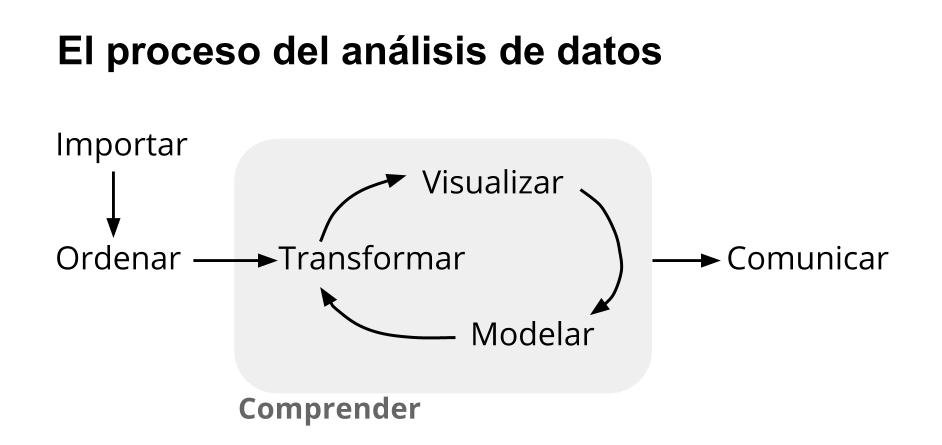
\includegraphics[width=6.28in]{imagenes/proceso_ciencia_datos} \caption{etapas en la aplicación de ciencia de datos}\label{fig:unnamed-chunk-2}
\end{figure}

Y todo ello llevado a cabo mediante la programación, por supuesto.

A lo largo de los capítulos de este libro vamos a aprender técnicas de
programación que nos permitan atravesar cada uno de los pasos del
proceso, y al hacerlo estaremos ejercitando las cuatro habilidades que
involucra la ciencia de datos.

Allá vamos.

\chapter{Una presentación a toda marcha de
R}\label{una-presentacion-a-toda-marcha-de-r}

Placeholder

\section{Nuestro primer proyecto en
R}\label{nuestro-primer-proyecto-en-r}

\subsection{A investigar: ¿Cual es la diferencia en mortalidad infantil
entre el sur y el norte de la Ciudad Autónoma de Buenos
Aires?}\label{a-investigar-cual-es-la-diferencia-en-mortalidad-infantil-entre-el-sur-y-el-norte-de-la-ciudad-autonoma-de-buenos-aires}

\subsection{Crear un proyecto en
RStudio}\label{crear-un-proyecto-en-rstudio}

\subsection{Escribiendo un script}\label{escribiendo-un-script}

\subsection{Cargar los datos}\label{cargar-los-datos}

\section{Visualización: la exploración gráfica de la
información}\label{visualizacion-la-exploracion-grafica-de-la-informacion}

\subsection{Haciendo mapas}\label{haciendo-mapas}

\subsection{Agregando datos}\label{agregando-datos}

\section{El veredicto final}\label{el-veredicto-final}

\subsection{¿Cuál es la diferencia en mortalidad infantil entre el sur y
el norte de la Ciudad Autónoma de Buenos
Aires?}\label{cual-es-la-diferencia-en-mortalidad-infantil-entre-el-sur-y-el-norte-de-la-ciudad-autonoma-de-buenos-aires}

\chapter{Poniendo los datos en forma}\label{poniendo-los-datos-en-forma}

Placeholder

\section{Primeros pasos al examinar un conjunto de datos
nuevo}\label{primeros-pasos-al-examinar-un-conjunto-de-datos-nuevo}

\section{\texorpdfstring{Cruzando variables: la operación
\texttt{join}}{Cruzando variables: la operación join}}\label{cruzando-variables-la-operacion-join}

\section{Transformando los datos}\label{transformando-los-datos}

\subsection{\texorpdfstring{Seleccionar columnas con
\texttt{select()}}{Seleccionar columnas con select()}}\label{seleccionar-columnas-con-select}

\subsection{\texorpdfstring{Filtrar filas con
\texttt{filter()}}{Filtrar filas con filter()}}\label{filtrar-filas-con-filter}

\subsubsection{Comparaciones}\label{comparaciones}

\subsubsection{Operadores lógicos}\label{operadores-logicos}

\subsection{\texorpdfstring{Ordenar filas con
\texttt{arrange()}}{Ordenar filas con arrange()}}\label{ordenar-filas-con-arrange}

\subsubsection{Valores faltantes}\label{valores-faltantes}

\subsection{\texorpdfstring{Agregar nuevas variables con
\texttt{mutate()}}{Agregar nuevas variables con mutate()}}\label{agregar-nuevas-variables-con-mutate}

\subsection{\texorpdfstring{Extraer sumarios con
\texttt{summarise()}}{Extraer sumarios con summarise()}}\label{extraer-sumarios-con-summarise}

\subsection{\texorpdfstring{¡BONUS! El operador ``pipe'':
\texttt{\%\textgreater{}\%}}{¡BONUS! El operador pipe: \%\textgreater{}\%}}\label{bonus-el-operador-pipe}

\chapter{Visualización}\label{visualizacion}

Placeholder

\section{\texorpdfstring{Una buena visualización para empezar: el
\emph{scatterplot}}{Una buena visualización para empezar: el scatterplot}}\label{una-buena-visualizacion-para-empezar-el-scatterplot}

\section{Ajustando color y tamaño}\label{ajustando-color-y-tamano}

\section{Facetado}\label{facetado}

\section{Gráficos de barras}\label{graficos-de-barras}

\section{Histogramas}\label{histogramas}

\section{Preparando una visualización para
compartir}\label{preparando-una-visualizacion-para-compartir}

\section{Otras visualizaciones}\label{otras-visualizaciones}

\chapter{Modelado estadístico}\label{modelado-estadistico}

Placeholder

\section{Regresión lineal simple}\label{regresion-lineal-simple}

\subsection{Regresión con una variable
numérica}\label{regresion-con-una-variable-numerica}

\subsection{Revolviendo los residuos}\label{revolviendo-los-residuos}

\subsection{Regresión con una variable
categórica}\label{regresion-con-una-variable-categorica}

\section{Regresión con múltiples
variables}\label{regresion-con-multiples-variables}

\chapter{Información geográfica y
mapas}\label{informacion-geografica-y-mapas}

Placeholder

\section{Los datos georreferenciados}\label{los-datos-georreferenciados}

\section{Formatos de archivo}\label{formatos-de-archivo}

\section{Explorando un archivo con información
geográfica}\label{explorando-un-archivo-con-informacion-geografica}

\section{Visualizando información
geográfica}\label{visualizando-informacion-geografica}

\section{Volcando en el mapa información de múltiples
fuentes}\label{volcando-en-el-mapa-informacion-de-multiples-fuentes}

\section{Combinando capas
geográficas}\label{combinando-capas-geograficas}

\bibliography{book.bib,packages.bib}


\end{document}
